\chapter{BASS and their Origins}

The main proposal in this work is the use of a BASS model as the surrogate model in the framework of Bayesian Optimization rather than a traditional Gaussian Process. To understand this method and why it is useful for this purpose, we develop first the theory that lead to the construction of this method, and then explain its behaviour in some detail. 

As with most other algorithms used for regression tasks, BASS is built upon a rich history of work that was previously done in the field. It begins with CART and decision trees, which MARS models are based on, and in turn BMARS (Bayesian MARS) uses the same model form as MARS but builds the model using the traditional Bayesian approach of defining a prior and constructing from there. Finally, BASS is a specific case of the BMARS model. This is much more clear when viewed as a diagram, as shown in the following figure. 

\begin{figure}[h]
	
\includegraphics[width=4cm]{Figures/missing.png}
	\centering
	\caption{The theoretical basis for BASS.}
	\label{building_BASS}
\end{figure}

\section{Decision Trees}

Decision trees are a fundamental and versatile tool that comes in two main flavours: classification trees and regression trees. These two types of trees serve distinct purposes and are employed to make predictions in different contexts. The term "Classification and Regression Tree" (CART) analysis serves as an umbrella term that encompasses both classification and regression tree procedures. CART was first introduced by Breiman et al. in 1984 \cite{breiman2017classification}, and it represents a unified framework for decision tree modelling, allowing for flexibility in handling both classification and regression tasks within the same algorithm. While classification and regression trees share common principles, such as recursive binary splitting and impurity measures (e.g., Gini impurity for classification and mean squared error for regression), they also exhibit some differences in terms of the criteria used to determine the best feature and split point at each node. The final predictions for a new data point are obtained by traversing the tree from the root node to a leaf node and returning the average (for regression) of the target variable for the training samples in that leaf node.

\begin{figure}[h]
	
\includegraphics[width=4cm]{Figures/missing.png}
	\centering
	\caption{A decision tree.}
	\label{building_BASS}
\end{figure}

In classification tree analysis, the primary objective is to predict the discrete class or category to which a given data point belongs. The decision tree algorithm partitions the data into subsets based on input features and assigns each data point to a specific class by following a path through the tree.

On the other hand, regression tree analysis is employed when the predicted outcome is a continuous, real-valued number. Similar to classification trees, regression trees partition the data based on input features. However, in this context, the goal is to estimate a numeric value for each data point, typically by computing the average of the target variable within each leaf node.

In both cases, the decision tree serves as a transparent and interpretable model, making it valuable for exploratory data analysis and predictive modelling. The tree's structure allows for a straightforward understanding of how decisions are made, and predictions for new data points are obtained by navigating the tree from the root node to an appropriate leaf node, where the final prediction is based on the characteristics of the training samples within that leaf.

The versatility and comprehensibility of decision trees have contributed significantly to their widespread use in various fields, and the distinctions between classification and regression trees make them adaptable tools for addressing a wide range of data analysis and prediction tasks. One problem that these methods tend to have though is overfitting, since if we allow the model to keep generating new nodes or leafs, the tree ultimately becomes too complex and every data point that we would like to analyse is simply too narrow to be useful as an aggregation scheme. 

While decision trees are useful on their own their real power comes from the versatility they provide, leading to a wide range of methods being born from the basic idea of splitting decisions into paths. These methods are sometimes called \textit{ensemble} methods, because they involve the creation and combination of multiple models to form a more robust and accurate predictive model. As an interesting side note, the term ensemble is borrowed from the world of music and theatre. Instead of relying on a single predictive model, these models create an ensemble of multiple models, each of which may have its own strengths and weaknesses. These individual models, often referred to as base models or weak learners, are combined in a way that leverages their collective intelligence to make better predictions.

Ensemble methods work on the premise that combining diverse models can reduce the risk of overfitting, enhance generalization, and improve predictive accuracy. Each model in the ensemble may make errors on some portions of the data, but by aggregating their predictions, the ensemble can produce more accurate and stable results. Common ensemble methods include Random Forest, Gradient Boosting, Adaptive Boosting, Bagging, and many others. The difference in these models is how they combine these different decision trees to achieve a more stable model. 

\section{MARS Models}

Now, let's shift our focus the following technique down the chain for us known as MARS, which stands for Multivariate Adaptive Regression Splines. MARS builds upon the foundation laid by decision trees but introduces a different paradigm for modelling complex relationships within data. Rather than using piecewise constant approximations, MARS leverages piecewise linear functions, thereby extending the toolbox of non-linear regression methods.

MARS is particularly valuable when the relationships between input features and the target variable are not strictly linear but can be approximated as a series of linear segments. Let's delve into the mathematical foundations of MARS to gain a deeper understanding.

For the following section, we will adopt the terminology and follow the development presented in \cite{Friedman_1991} and \cite{friedman1991multivariate}.

MARS is defined using functions that are piecewise linear in the form of $(x - t)+$ and $(t - x)+$. These functions take the maximum between 0 and the value within the function, as follows:

$$
(x - t)_+ = \max\{ 0, x - t \}= \begin{cases} 
	x - t &\mbox{if } x > t, \\
	0 & \mbox{if } x \leq t. \end{cases}
$$

Each function is piecewise linear with a slope change at the value $t$, which makes them linear splines. Each pair divided at the value $t$ is referred to as a \say{reflected pair}. The idea of the method is to form reflected pairs for each input variable $X_j$ with slope changes a selection of observed values $x_{ij}$. Following this construction and considering a variable $X_j$, the collection of basis functions is:
$$
\mathcal{C} = \{ (X_j - t)_+, (t - X_j)_+ \}, \text{ with } t \in \{ x_{1,j}, x_{2,j}, \ldots x_{N,j} \}, \text{ y } \,\, j = 1,2, \ldots , p.
$$
And each reflected pair appears as follows, and are shown in figure \ref{reflected_pairs}: 
$$
h_1(X) = h(X_j - x_{ij}) 
$$
$$
h_2(X) = h(x_{i,j} - X_j)
$$
\begin{figure}[h]
	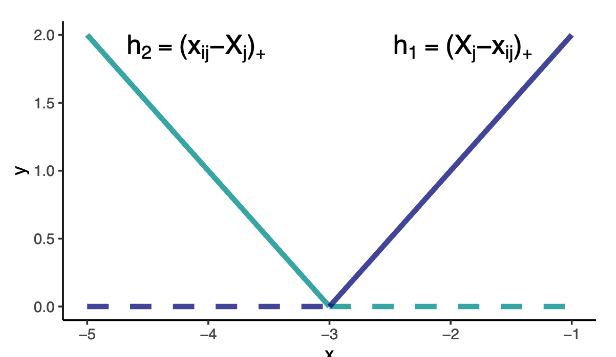
\includegraphics[width=10cm]{Figures/3ref_pair.png}
	\centering
	\caption{The constructed reflected pairs.}
	\label{reflected_pairs}
\end{figure}
So, for each $X_j$, the set of candidate reflected pairs that exist at each of the $x_{ij}$ points of that variable is shown in figure \ref{hinges}. 
\begin{figure}[h]
	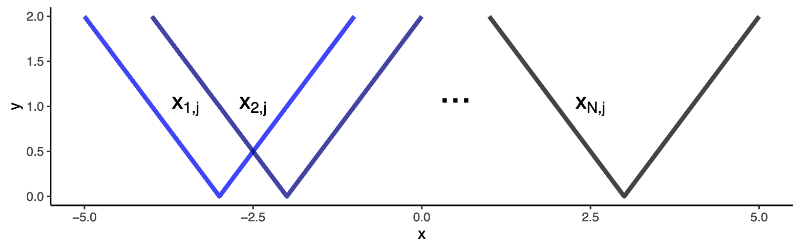
\includegraphics[width=10cm]{Figures/3hinge.png}
	\centering
	\caption{Collections of hinge functions.}
	\label{hinges}
\end{figure}

This means that if all input values are distinct, there are a total of $2Np$ basis functions, and $2N$ divisions in each of the splines for each variable. The model we use to combine all variables is an additive one in $\boldsymbol\beta$:
$$
f(X) = \beta_0 + \sum_{m=1}^M \beta_m h_m(X),
$$
where each function $h_m(X)$ is an element of $\mathcal{C}$ or a linear combination of these basis functions. For this initial explanation, we will use only functions that do not involve interactions (the model with interactions works very similarly to CART decision trees).

The model construction process (denoted as $\mathcal{M}$) begins with the base model $\hat f(X) = \hat \beta_0 = h_0(X) = 1$, where a term functioning as an intercept at the origin is defined. To add terms incrementally, all functions in the set $\mathcal{C}$ are candidates for entry into $\mathcal{M}$. For each observation $x_{ij}$, the new model involving these functions is fitted as follows:
$$
\hat f(X) = \hat \beta_0 + \hat \beta_1 h_1(X) + \hat \beta_2 h_2(X).
$$
Since this is a linear form in terms of each of the functions $h_i$, the adjustment of each parameter $\hat \beta_i$ is done by minimizing the sum of squares.

The reflected pair that is added is the one that minimizes the training error. This process is repeated for each of the remaining reflected pairs, solving OLS to determine the new $\boldsymbol\beta$, and adding the one that continues to minimize the error. The stopping criterion can be either that none of the remaining reflected pairs reduces the error enough (in absolute or relative terms) or until we have a predetermined number of variables in the model.

This leads to overfitting the data, but this is the goal in this part of the procedure when minimizing the training error. Once we have $\mathcal{M}$, we start the second part of model fitting, which is the pruning part. In this case, terms $h_i(X)$ are removed iteratively, starting with the one that produces the smallest increase in the residual sum of squares when removed. This procedure yields a better model for each $\lambda$ size, denoted as $\hat f_\lambda$.

Several procedures can be used to estimate the optimal value of $\lambda$, such as cross-validation or bootstrap, but this involves a significant computational cost. To minimize this cost, MARS models generally use a generalized cross-validation (GCV) procedure. This criterion is defined as:
$$
GCV(\lambda) = \frac{ \sum_{i=1}^N (y_i - \hat f_\lambda(x_i))^2 }{\left( \frac{1 - M(\lambda)}{N} \right)^2},
$$
where the value $M(\lambda)$ is the number of effective parameters in the model, depending on the number of terms plus the number of breakpoints used, penalized by a factor (this factor is 2 in the case for additive in $X$ that we are explaining, and 3 when there are interactions).

Now that we have described the base model, we can go back and consider the differences when incorporating interaction terms. Instead of just adding terms additively, products between the existing $h_\ell$ functions in the model and between each reflected pair of each $x_{ij}$ can be added. Note that this general case encompasses the previous one because if you want to add a reflected pair without interacting with the other variables, you simply multiply by $h_0 = 1$.

In this way, a model $\mathcal{M}$ with $M$ terms will be updated as follows after finding the combination $\hat \beta_{M+1} h_\ell(X) \cdot (X_j - t)+ + \hat \beta{M+2} h_\ell(X) \cdot (t-X_j)_+$ that best minimizes the training error:
$$
\hat f(X) = \hat \beta_0 + \sum_{m=1}^M \hat \beta_m h_m(X) + \hat \beta_{M+1} h_\ell(X) \cdot (X_j - t)_+ + \hat \beta_{M+2} h_\ell(X) \cdot (t-X_j)_+,
$$
where $h_\ell \in \mathcal{M}$ and $t = x_{ij}$ for any case. \textcolor{red}{Como transiciono de una idea a otra aqui?}

One interesting consideration is that the added flexibility of these models does not end with it being piecewise linear, as one small alteration that can be made is to replace the truncated linear functions with truncated cubic basis functions or other functions of a higher order, which provides allows the resulting model to be fully differentiable within its domain. 

In conclusion, our exploration of Multivariate Adaptive Regression Splines (MARS) is a powerful and versatile technique for modelling complex relationships within data. Unlike traditional linear regression, MARS leverages piecewise linear functions, making it a valuable tool when dealing with non-linear relationships between input features and the target variable. The methodology behind MARS involves the creation of reflected pairs and the incremental addition of basis functions to the model, effectively adapting to the data's intricacies. The model construction process aims to minimize the training error by iteratively selecting the reflected pair that provides the most significant reduction in error. This leads to a model that can potentially overfit the data, but this is by design during the training phase. Subsequently, a pruning step is employed to refine the model, removing terms that do not contribute significantly to the model's predictive power.

\section{BMARS Models}

The key innovation that distinguishes BMARS from its predecessor lies in its Bayesian framework. While MARS primarily focuses on constructing piecewise linear models by iteratively selecting basis functions to minimize training error, BMARS introduces Bayesian methods to bring a probabilistic perspective into this process. This integration of Bayesian principles allows BMARS to provide not only point estimates of model parameters but also entire probability distributions, enabling a more comprehensive understanding of the uncertainty inherent in the modelling process.

As described in \cite{denison1998bayesian}, which is the original paper where this method was proposed, the idea behind this model is to allow more flexibility in the traditional MARS model by looking at it from a Bayesian perspective. This is done by mimicking the MARS model with changes in framing, namely by considering the number of basis functions, along with their \textit{type}, their coefficients and their form (the positions of the split points and the sign indicators) as random. 

We take the definition of a basis type from the original paper and a small example from there to make the definition tangible, and include it here for completeness. 
\begin{definition}
	We consider basis functions $X_i$ and $X_j$ to be of the same type if $[x(1,i), \ldots, x(J_i,i)]$ is identical to some permutation of $[x(1,j), \ldots, x(J_j,j)]$. Hence, with $m$ predictor variables, there are $N$ different types of basis functions, where $N$ is given by:
	\begin{equation}
		N = \sum_{i=1}^{m} \binom{m}{i} = 2^m - 1. \label{eq3}
	\end{equation}	
\end{definition}

Note that the sum does not include the constant basis function term (for which $i$ would equal 0 in \eqref{eq3}), as this basis $X_1$ is always the sole constant basis function in the model, so it cannot be chosen as a candidate basis. Frequently, some maximum order of interaction $I$ is assigned to the model, such that $J_i \leq I$ for $i = 1, \ldots, k$. In which case, the sum in \eqref{eq3} only runs from 1 up to $I$. We let $T_i \in \{1, 2, \ldots, N\}$ denote the type of basis function $X_i$; thus, $T_i$ effectively tells us which predictor variables we are splitting on, i.e., what the values of $x(1,i), \ldots, x(J_i,i)$ are.

As an example, suppose we have a problem with just two predictors, i.e., $m = 2$. Then the types of basis functions that could be in the model (not including the constant one) are $[\pm (x_1 - \ast)]$ (say, type 1), $[\pm (x_2 - \ast)]$ (say, type 2), and $[\pm (x_1 - \ast)][\pm (x_2 - \ast)]$ (say, type 3). So for all those basis functions which split only on predictor $x_2$, their types $T_i$ are all equal to 2.

The key insight that this framework of construction is based on is that any MARS model can be uniquely defined by the following: 
\begin{itemize}
	\item The number of basis functions $k$, 
	\item the coefficients of the basis functions $a_i$, 
	\item the type of basis functions $T_i$, 
	\item the knot points associated with each interacting term $t_{ji}$, 
	\item the sign indicators associated with each interacting term $s_{ji}$. 
\end{itemize}
and as such, a probability distribution over the possible MARS models can be constructed, enabling a more comprehensive understanding of the uncertainty inherent in the modelling process since the response is an entire probability distribution rather than a single model. This framework also provides the ability to do ANOVA and Sobol decompositions for sensitivity analysis. One important aspect of this framework for construction is that the number of parameters varies with the number of basis functions $k$, and as such, a traditional method such as Markov chain Monte Carlo cannot be used directly, as it assumes constant parameters. An extended version of MCMC is therefore used, called reversible jump MCMC (first introduced in \cite{green1995reversible}), that allows for a variable number of parameters. \textcolor{red}{Cual es el modelo? Tengo el paper pero no lo veo claro.}

\section{BASS Models}

Bayesian Adaptive Spline Surface (BASS) models are an extension of the family of non parametric regression models of which multivariate adaptive regression splines (MARS) was the first developed in 1991 and is the most basic \cite{friedman1991multivariate}. MARS is an extension of linear models, where interactions between variables and non linearities are modelled automatically. 

The extension of this model of interest is the BMARS model. As the authors state in \cite{denison1998bayesian}, the aim of BMARS is to provide a Bayesian model that mimics the MARS procedure. This is done by considering the number of basis functions, along with their type, the coefficients and their form, random. Then, a suitable MCMC algorithm, in this case reversible jump monte carlo \cite{green1995reversible}, is used to calculate a suitable posterior for the problem. The great advantage to RJMCMC over other MCMC techniques is that the number of parameters can be variable, and as such, is a great basis for the type of analysis that is necessary for models in the MARS class. 

BASS models are an adaptation of BMARS models that include some efficiency improvements for posterior sampling alongside parallel tempering for better posterior exploration \cite{francom2020bass}. For our purposes though, the most significant improvement is that it allows the use of categorical variables alongside some continuous variables. This is incredibly useful in the context of hyper-parameter optimization, where there are generally some categorical variables such as polynomial degree, smoothing, etc. While we remain in the one dimensional case and this improvement is not necessarily useful, the multi dimensional case will benefit greatly from this improvement. 

A detailed rundown of the model, its priors, and its construction in general can be seen in \cite{francom2020bass}, but, we include the definition of the model presented in that work for completeness. 

Let $y_i$ denote the dependent variable and $\boldsymbol{x}_i$ denote a vector of $p$ independent variables, with $i = 1, \ldots, n$. Without loss of generality, let each independent variable be scaled to be between
zero and one. We model $y_i$ as 
\[ y_i = f(\boldsymbol{x}_i) + \epsilon_i, \, \, \epsilon_i \sim \mathcal{N}(0,\sigma^2) \]
\[ f(\boldsymbol{x}) = a_0 + \sum_{m=1}^{M} a_m B_m(\boldsymbol{x}) \]
\[ B_m(\boldsymbol{x}) = \prod_{k=1}^{K_m} g_{km} [s_{km}(\boldsymbol{x}_{v_{km}} - t_{km}) ]^\alpha_+ \]

The only difference between this setup and that of MARS and BMARS is the inclusion of the constant $g_{km}$ in each element of the tensor product. This term is $g_{km}=[s_{km}(\boldsymbol{x}_{v_{km}} - t_{km}) ]^\alpha_+$, where $s_{km} \in \{-1,1\}$ is referred to as the sign, $t_{km}\in [0,1]$ is a knot, $v_{km}$ selects a variable, $K_m$ is the degree of interaction, and $\alpha$ determines the degree of the polynomial splines. This normalizes the basis functions so that the basis coefficients $a_1, \ldots, a_M$ are on the same scale, making computations more stable.

